\chapter{Base Tracking}\label{chap:base_tracking}


\section{Extended Kalman Filter}
One part of the work is focused on the estimation of the state of the moving platform.
An Extended Kalman Filter is design in order to have the most reliable value of the state of the platform.

Kalman filtering is an algorithm that uses a series of noisy measurements observed over time and produces estimates of unknown variables that tend to be more precise than those based on a single measurement alone, by using Bayesian inference and estimating a joint probability distribution over the variables for each time frame.\\
The algorithm works in a two-step process:
\begin{itemize}
\item In the prediction step, the Kalman filter produces estimates of the current state variables, along with their uncertainties, based on a model of the system:
\begin{equation}
\boldsymbol{x}_k = f(\boldsymbol{x}_{k-1},\boldsymbol{u}_k) + \boldsymbol{w}_k
\end{equation}
\item Once the outcome of the next measurement is observed:
\begin{equation}
\boldsymbol{z}_k = h(\boldsymbol{x}_{k}) + \boldsymbol{v}_k
\end{equation}
these estimates are updated using a weighted average, with more weight being given to estimates with higher certainty.
\end{itemize}
In the extended Kalman filter, the state transition and observation models don't need to be linear functions of the state but may instead be differentiable functions.\\
($\boldsymbol{w}_k$ and $\boldsymbol{v}_k$ are the process and observation noises which are both assumed to be zero mean multivariate Gaussian noises with covariance $\boldsymbol{Q}_k$ and $\boldsymbol{R}_k$ respectively. $\boldsymbol{u}_k$ is the control vector).

  The algorithm is recursive. It can run in real time, using only the present input measurements and the previously calculated state and its uncertainty matrix; no additional past information is required.\\
The Kalman filter does not require any assumption that the errors are Gaussian. However, the filter yields the exact conditional probability estimate in the special case that all errors are Gaussian-distributed.\\
Initialization
\begin{align}
\begin{split}
\boldsymbol{x}_{0|0} = x_0\\
\boldsymbol{P}_{0|0} = P_0
\end{split}
\end{align}
In this case the prediction equations are continuous in time, so for the prediction step of the EKF we have to solve:
\begin{align}
\begin{split}
\boldsymbol{\dot{\hat{x}}}(t) &= f(\boldsymbol{\hat{x}}(t),\boldsymbol{u}(t)) \\
\boldsymbol{\dot{P}}(t) &= \boldsymbol{F}(t) \boldsymbol{P}(t) + \boldsymbol{P}(t)\boldsymbol{F}(t)^{\top } + \boldsymbol{Q}(t)
\end{split}
\end{align}
for $t \in (t_{k-1}, t_k)$ where %TODO
\begin{align}
\begin{split}
\boldsymbol{\hat{x}}(t_{k-1}) &= \hat{x}_{k-1|k-1} \\
\boldsymbol{P}(t_{k-1}) &= P_{k-1|k-1}
\\
{\boldsymbol{F}}(t)&=\left.{\frac  {\partial f}{\partial {\boldsymbol{x}}}}\right\vert _{{{\hat  {{\boldsymbol{x}}}}(t),{\boldsymbol{u}}(t)}}  \\
\boldsymbol{\hat{x}}_{k|k-1} &= \boldsymbol{\hat{x}}(t_{k}) \\
\boldsymbol{P}_{k|k-1} &= \boldsymbol{P}(t_{k})
\end{split}
\end{align}
In order to save some computation we can discretize the dynamicin order to have shorter computation during the prediction step of the EKF:
\begin{align}
\begin{split}
\boldsymbol{\hat{x}}_{k|k-1} &= f(\boldsymbol{\hat{x}}_{k-1|k-1},\boldsymbol{u}_k) \\
\boldsymbol{P}_{k|k-1} &= \boldsymbol{F}_{k-1} \boldsymbol{P}_{k-1|k-1}\boldsymbol{F}_{k-1}^{\top } + \boldsymbol{Q}_{k}
\end{split}
\end{align}
where the state transition matrix is defined to be the following Jacobians:
\begin{align}
\begin{split}
\boldsymbol{F}_{k-1}&= \left.{\frac{\partial f}{\partial {\boldsymbol{x}}}} \right \vert_{\hat{\boldsymbol{x}}_{k-1|k-1},\boldsymbol{u}_{k}} 
\end{split}
\end{align}
While the update equations are discrete in time and they yield to the following update step: 
\begin{align}
\begin{split}
\boldsymbol{K}_{k} &= \boldsymbol{P}_{k|k-1} \boldsymbol{H}_{k}^{\top }(\boldsymbol{H}_{k} \boldsymbol{P}_{k|k-1} \boldsymbol{H}_{k}^{\top }+ \boldsymbol{R}_{k})^{-1}
\\
\hat{\boldsymbol{x}}_{k|k} &= \hat{\boldsymbol{x}}_{k|k-1} + \boldsymbol{K}_{k} (\boldsymbol{z}_{k}-h(\hat{\boldsymbol{x}}_{k|k-1}))
\\
\boldsymbol{P}_{k|k} &=(\boldsymbol{I}-\boldsymbol{K}_{k}\boldsymbol{H}_{k})\boldsymbol{P}_{k|k-1}
\end{split}
\end{align}
where the observation matrix is defined to be the following Jacobian:

\begin{align}
\begin{split}
\boldsymbol{H}_{k} = \left.{\frac{\partial h}{\partial {\boldsymbol{x}}}} \right \vert_{\hat{\boldsymbol{x}}_{k|k-1}}
\end{split}
\end{align}

\section{Prediction update: non-holonomic model}
The platform is considered as a car and simulated with a non-holonomic model. 
In this model the state is defined as $\boldsymbol{x} = (x, y, z,\theta , v, \phi)$:
It corresponds to the 3 position in a space $(x,y,z)$ and the yaw angle of the platform $(\theta)$ w.r.t. the world frame, the forward velocity ($v$) and the angle of the front wheels ($\phi$). The system depends on a parameter $L$ that corresponds to the distance between the front and the back wheels.\\
In this model the control input are the change in velocity $v$ and in the angle of curvature $\phi$. \\
The equation of motion in continuous time are:
\begin{align}
\boldsymbol{\dot{x}} = f(\boldsymbol{x},\boldsymbol{u}) \nonumber
\end{align}
\begin{align}
\begin{split}
\dot{x} &= v cos(\theta) \\
\dot{y} &= v sin(\theta) \\
\dot{z} &= 0 \\
\dot{\theta} &= \frac{v}{L}tan(\phi)\\
\dot{v} &= u_1 \\
\dot{\phi} &= u_2 
\end{split}
\end{align}
It is possible to discretize these dynamics in $t \in (t_{k-1}, t_k)$ with a first order finite difference:
\begin{align}
\boldsymbol{\dot{x}} \approx \frac{\boldsymbol{x}_k - \boldsymbol{x}_{k-1} }{dt} \approx f(\boldsymbol{x}_{k-1},\boldsymbol{u}_k) \nonumber
\end{align}
with $\boldsymbol{x}_k = \boldsymbol{x}(t_k)$, $\boldsymbol{x}_{k-1} = \boldsymbol{x}(t_{k-1})$, $dt = t_k - t_{k-1}$
\begin{align}
\begin{split}
x_k &= x_{k-1} + dt \big(v_{k-1} cos(\theta_{k-1})\big) \\
y_k &= y_{k-1} + dt \big(v_{k-1} sin(\theta_{k-1})\big) \\
z_k &= z_{k-1} \\
\theta_k &= \theta_{k-1} + dt\Big(\frac{v_{k-1}}{L}tan(\phi_{k-1}) \Big)\\
v_{k} &= v_{k-1} + dt \big(u_{1k}\big) \\
\phi_k &= \phi_{k-1} + dt \big(u_{2k}\big) 
\end{split}
\end{align}
In order to solve the former system, we have anyway to find a numerical solution. For this purpose we use a    
RUNGE-KUTTA scheme %TODO
\begin{figure}[!ht]
    \centering
    \includegraphics[width=0.5\textwidth]{img/non_holonomic_model.png}
    \caption{Non-holonomic model}
    \label{fig:nonholonomicmodel}
\end{figure}
\subsection{Straight and circular path}
For now we assume the input $u_1$ and $u_2$  are equal to zero, so the platform can be static ($v_f(0) = 0$) can move in a straight line ($v_f(0) \neq 0$ and $\phi(0) = 0$) or in a circle ($v_f(0) \neq 0$ and $\phi(0) \neq 0$)

\subsection{Infinity shape path}
In the MBZIRC challenge the moving platform will move in an infinity-shape path described in the figure \ref{fig:arenachallenge}. 
We need to describe in a mathematical way this shape in order to use this information in the prediction step of the EKF.
From the specification of the challenge:
\begin{itemize}
\item the car is moving with constant velocity $v$ along the path
\item the radius of the trajectory is $r$m
\item the path is making a cross in the middle that creates 4 angles of $\pi/2$ 
\end{itemize}
The easiest way to describe this path is to define how the angle $\theta$ is changing in function of the space. \\
It easy to see that the shape can be seen as a combination of a cross and two circles.
The cross is simply defined as the union between the two line:
\begin{align}
\begin{split}
y &= x \\
y &= -x
\end{split}
\end{align}
while the two circles 
\begin{align}
\begin{split}
y^2 + (x - x_0)^2 &= r^2 \\
y^2 + (x + x_0)^2 &= r^2 
\end{split}
\end{align}
It easy to see that if we want the intersections between these two functions to be exactly in the 4 points we have to choose 
\begin{align}
\begin{split}
x_0 = \frac{\sqrt{2}}{2}r
\end{split}
\end{align}
That correspond to the 4 intersections coordinate
\begin{align}
\begin{split}
\Big(\frac{\sqrt{2}}{2}r,\frac{\sqrt{2}}{2}r\Big);
\Big(\frac{\sqrt{2}}{2}r,-\frac{\sqrt{2}}{2}r\Big);
\Big(-\frac{\sqrt{2}}{2}r,-\frac{\sqrt{2}}{2}r\Big);
\Big(-\frac{\sqrt{2}}{2}r,\frac{\sqrt{2}}{2}r\Big)
\end{split}
\end{align}

\begin{figure}[!tbp]
  \centering
 {\includegraphics[width=0.48\textwidth]{img/constructionshape1_.png}\label{fig:constuctinfinity1}}
  \hfill
  {\includegraphics[width=0.48\textwidth]{img/constructionshape2_.png}\label{fig:constuctinfinity2}}
  \caption{How to construct the infinity-shape path}
\end{figure}

If we travel over the two circumferences the intersections correspond to angles $\theta = \pm \frac{3\pi}{4}$. \\
Now it is obvious to see that the path is symmetric and it can be divided in 4 parts and describing how the angle is changing in one of this section, the whole trajectory is defined.\\
We can observe that:
\begin{align}
\theta(x) =
\begin{cases}
    -\frac{x}{r}  &x\in \Big[0,\frac{3\pi}{4}r\Big] \quad \quad \ \ \  \\[10pt]
    -\frac{3\pi}{4} &x\in \Big[\frac{3\pi}{4}r ,\frac{3\pi}{4}r + r\Big]
\end{cases}
\end{align}
This function define a quarter of the trajectory \ref{fig:quarter_path} in function of the radius $r$ of the path.\\
It is now possible to use it to generate the entire trajectory $(x(t),y(t))$\ref{fig:entire_path}: we know that the length of the path is $l = 4(\frac{3\pi}{4}r + r)$ and given the constant velocity $v$ we can calculate the time to complete the trajectory $T = \frac{l}{v}$ and it is simple to define $\theta(t)$ just stretching or shrinking $\theta(x)$ .\\
So we can define
\begin{align}
\begin{split}
\dot{x} &= v cos(\theta(t)) \\
\dot{y} &= v sin(\theta(t))
\end{split}
\end{align}
And finally we have
\begin{align}
\begin{split}
x_k &= x_{k-1} + dt \big(v_{k-1} cos(\theta_{k-1})\big) \\
y_k &= y_{k-1} + dt \big(v_{k-1} sin(\theta_{k-1})\big)
\end{split}
\end{align}

\begin{figure}[!tbp]
  \centering
 {\includegraphics[width=0.8\textwidth]{img/angle_x.eps}\label{fig:quarter_theta}}
  \hfill
  {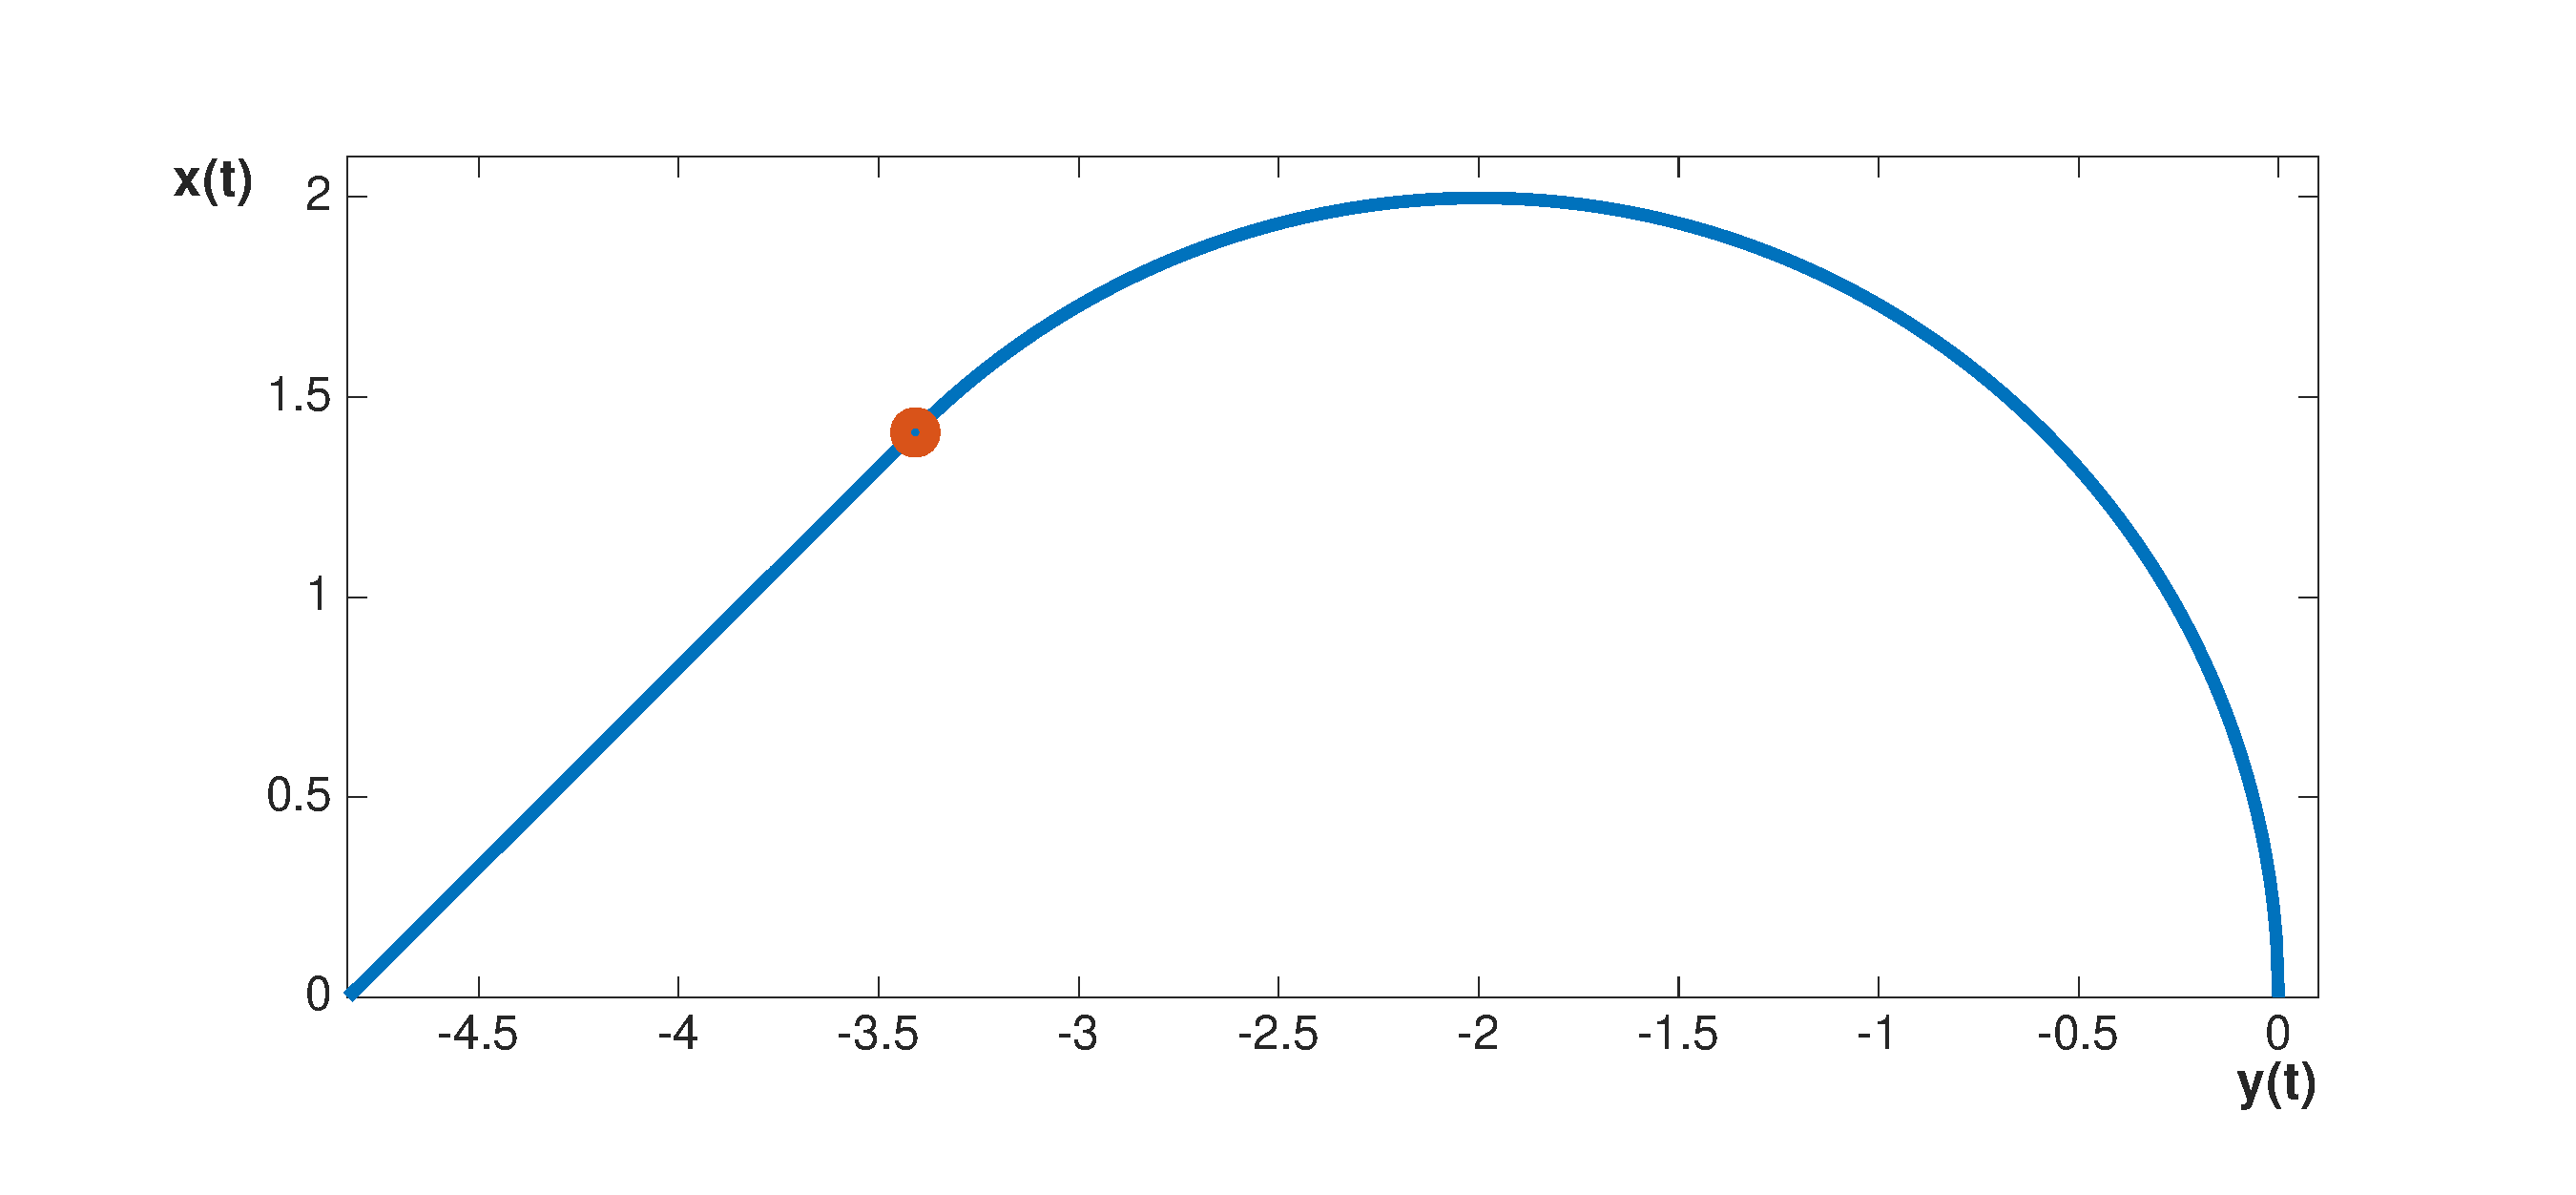
\includegraphics[width=0.8\textwidth]{img/path_x_quarter.eps}\label{fig:quarter_xy}}
  \caption{The parametrization of a quarter of the path}
  \label{fig:quarter_path}
\end{figure}

\begin{figure}[!ht]
    \centering
    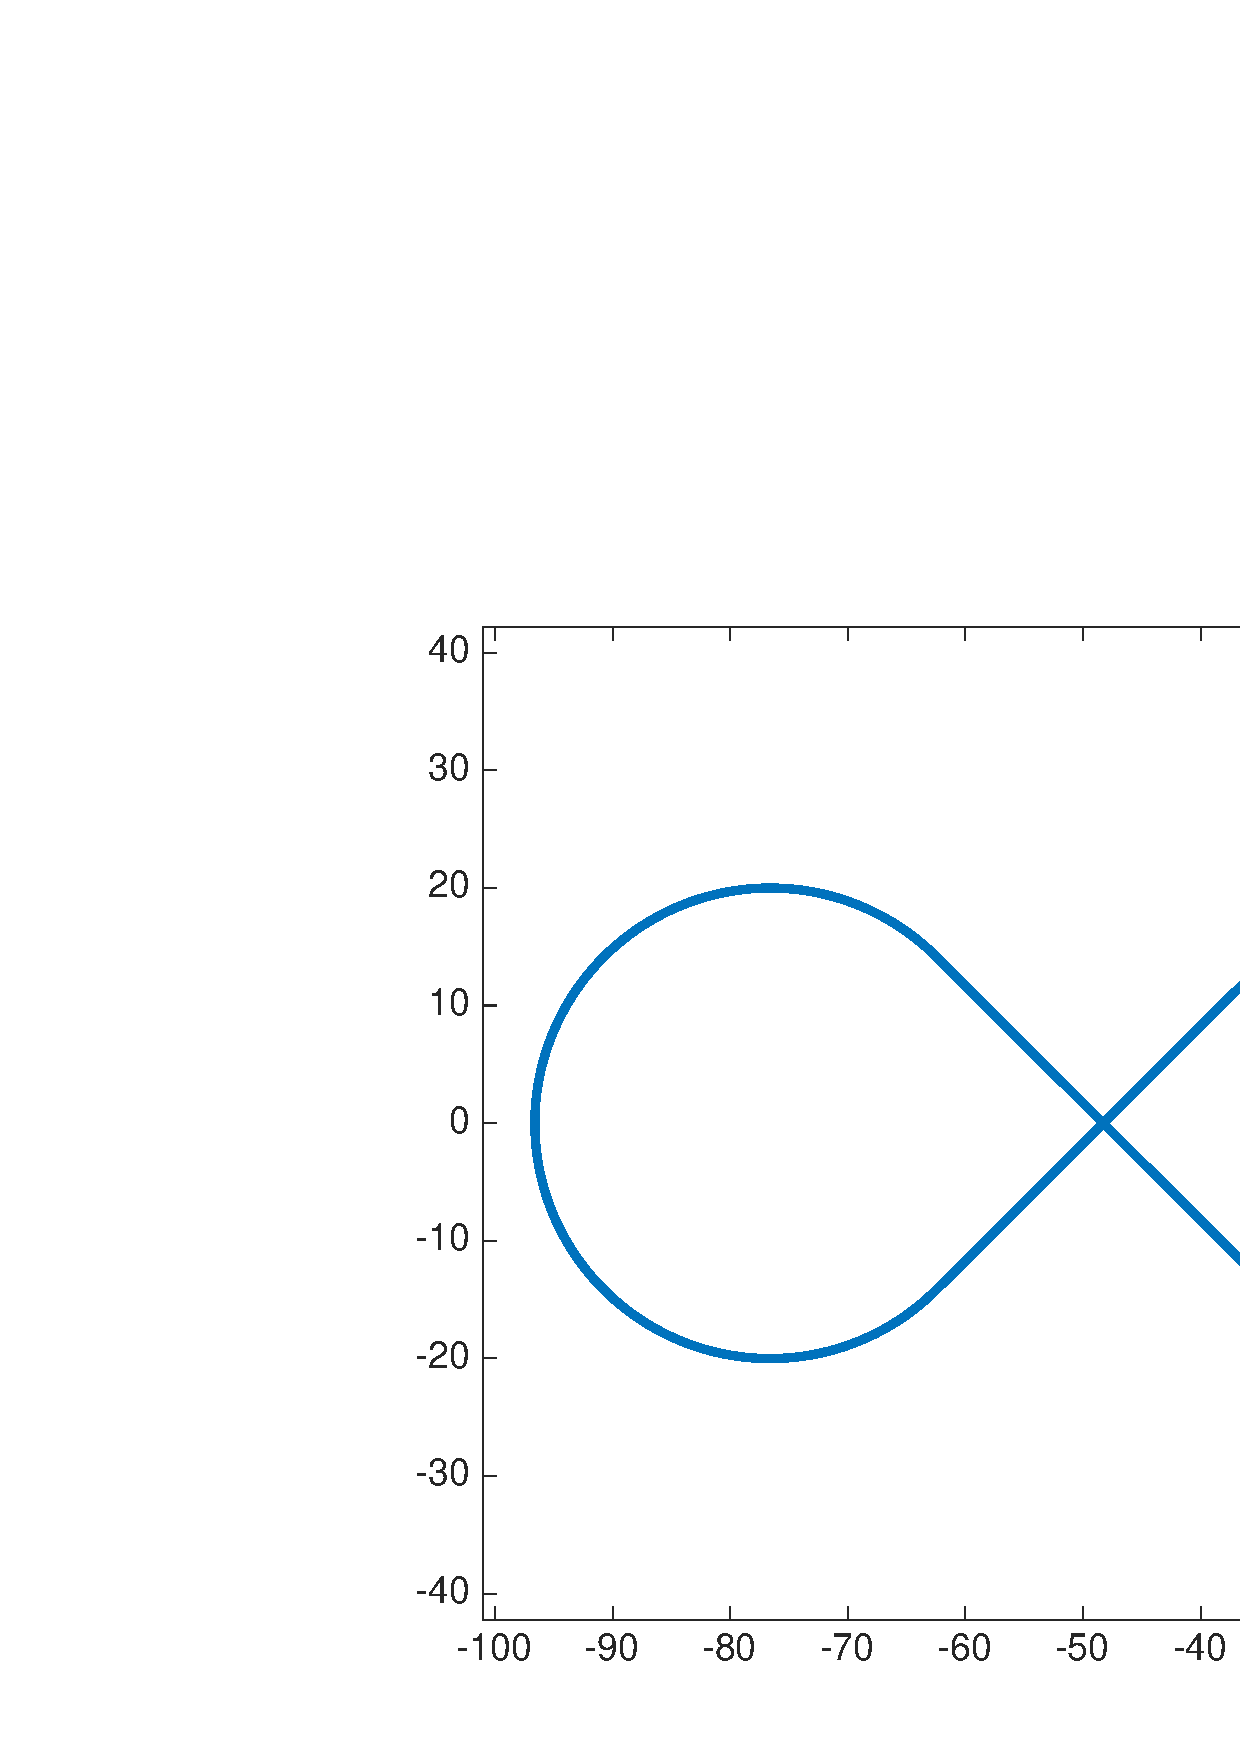
\includegraphics[width=1\textwidth]{img/infinityshapepath.png}
    \caption{Infinity-shape path}
    \label{fig:entire_path}
\end{figure}

\section{Measurement update}
\subsection{Tag Detector}
\subsubsection{Base design}
image

\subsubsection{April Tag vs Ar Sys}
precision comparison vs frequency
\subsubsection{Implementation}
nodlet
\subsection{Cross Detector}
pnp problem
\subsection{Covariance Estimation}



\section{Results}
\begin{figure}[!ht]
    \centering
    \includegraphics[width=0.97\textwidth]{img/position_real_world_fast.png}
    \caption{EKF 1}
    \label{fig:ekf_position_fast}
\end{figure}
\begin{figure}[!ht]
    \centering
    \includegraphics[width=0.97\textwidth]{img/position_simulation_hot_init.png}
    \caption{EKF 2}
    \label{fig:ekf_position_hot_init}
\end{figure}
